\footnotesize
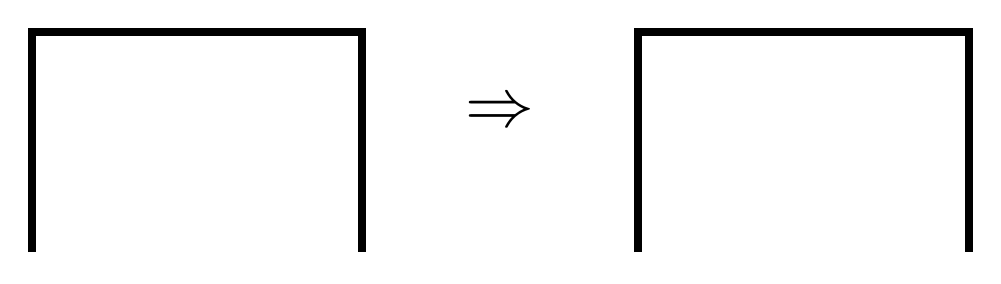
\begin{tikzpicture}[scale=.7]
\begin{scope}
\FixedSupport{0,0}
\FixedSupport{6,0}
\draw[line width=1mm](0,0)--++(0,4)--++(6,0)--++(0,-4);
\setstructmech{convention=direction}
\NodalForce{0,6}[N][-\SI{200}{\kn}][N]
\NodalForce{6,6}[N][-\SI{400}{\kn}][N]
\end{scope}
\begin{scope}[xshift=11cm]
\FixedSupport{0,0}
\FixedSupport{6,0}
\draw[line width=1mm](0,0)--++(0,4)--++(6,0)--++(0,-4);
\setstructmech{convention=direction}
\NodalForce{0,6}[N][-\SI{600}{\kn}][N]
\NodalForce{6,6}[N][-\SI{0}{\kn}][N]
\end{scope}
\node at(8.5,2.5){\Huge$\Rightarrow$};
\end{tikzpicture}